\documentclass[12pt,a4paper]{report}
\usepackage[utf8]{inputenc} % un package
\usepackage[T1]{fontenc} % un second package
\usepackage[francais]{babel} % un troisième package
\usepackage{color} % Package de la couleur
\usepackage{verbatim}
\usepackage{moreverb}
\usepackage{amsmath}
\usepackage{amsfonts}
\usepackage{amssymb}
\usepackage{graphicx}
\usepackage[top=2cm, bottom=2cm, left=2cm, right=2cm]{geometry}
\author{IMA World Health Web Developer Team}
\title{
\includegraphics[width=12cm]{ima.png} \\BASIC HOSPITAL INFORMATION MANAGEMENT APPLICATION\\ (BHIMA) \\ Manuel d'utilisation}

\begin{document}
%Page de garde
\maketitle 
\chapter{Présentation}
\section{Accès au système}
\large{Pour accéder au système, la première de chose à faire est de lancer un navigateur web, en suite saisir l'adresse web de server dans la barre d'adresse du navigateur.}

La première interface de l'application est un formulaire qui demande à chaque utilisateur de pouvoir fournir son login, son mot de passe mais aussi de spécifier  le projet dont il sont assigné, comme le montre le formulaire ci-dessous.
\begin{figure}[h]
\begin{center}
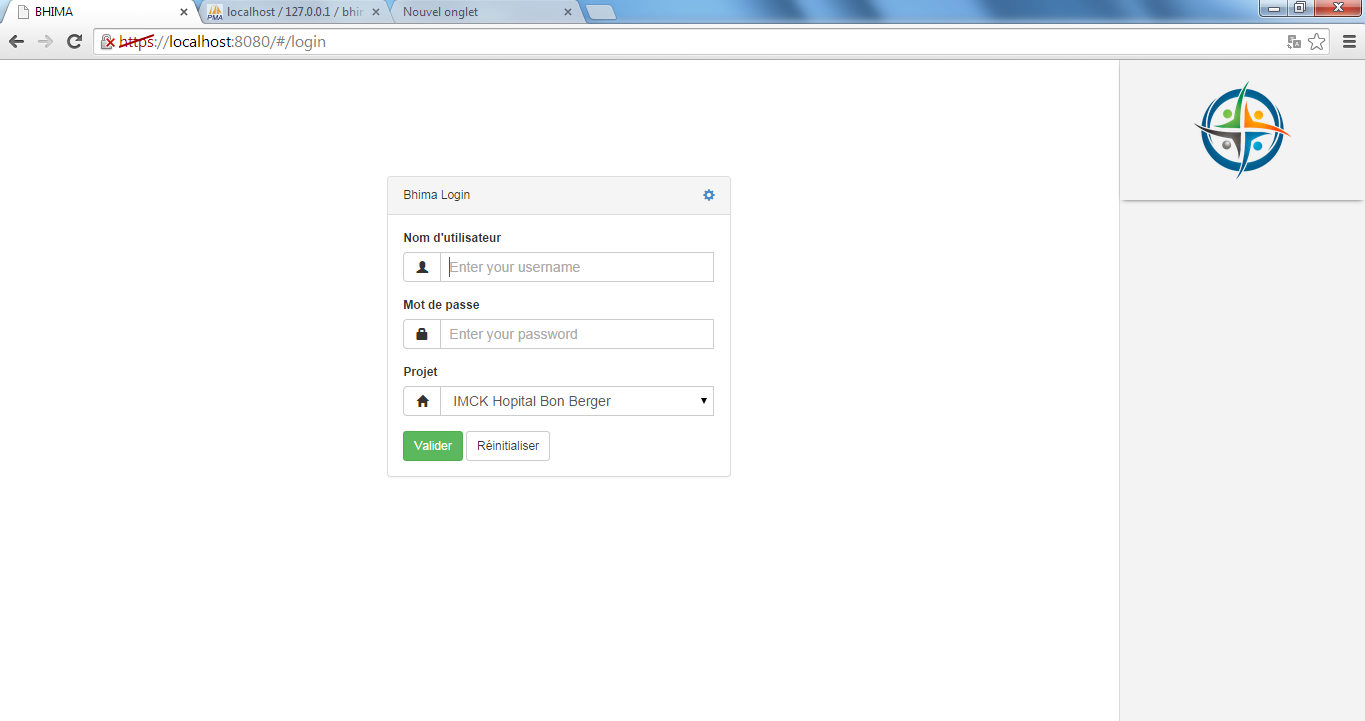
\includegraphics[width=12cm]{pic/login.png}
\end{center}
\caption{Page d'identification et authentification des utilisateurs}
\label{Page d'identification et authentification des utilisateurs}
\end{figure}
\\ L'accès au système n'est garanti que pour ceux qui possèdent un compte utilisateur, si l'utilisateur s'est authentifié alors il sera dirigé vers l'interface principale de l'application qui se présente de la manière suivante.
\newpage
\begin{figure}[h]
\begin{center} 
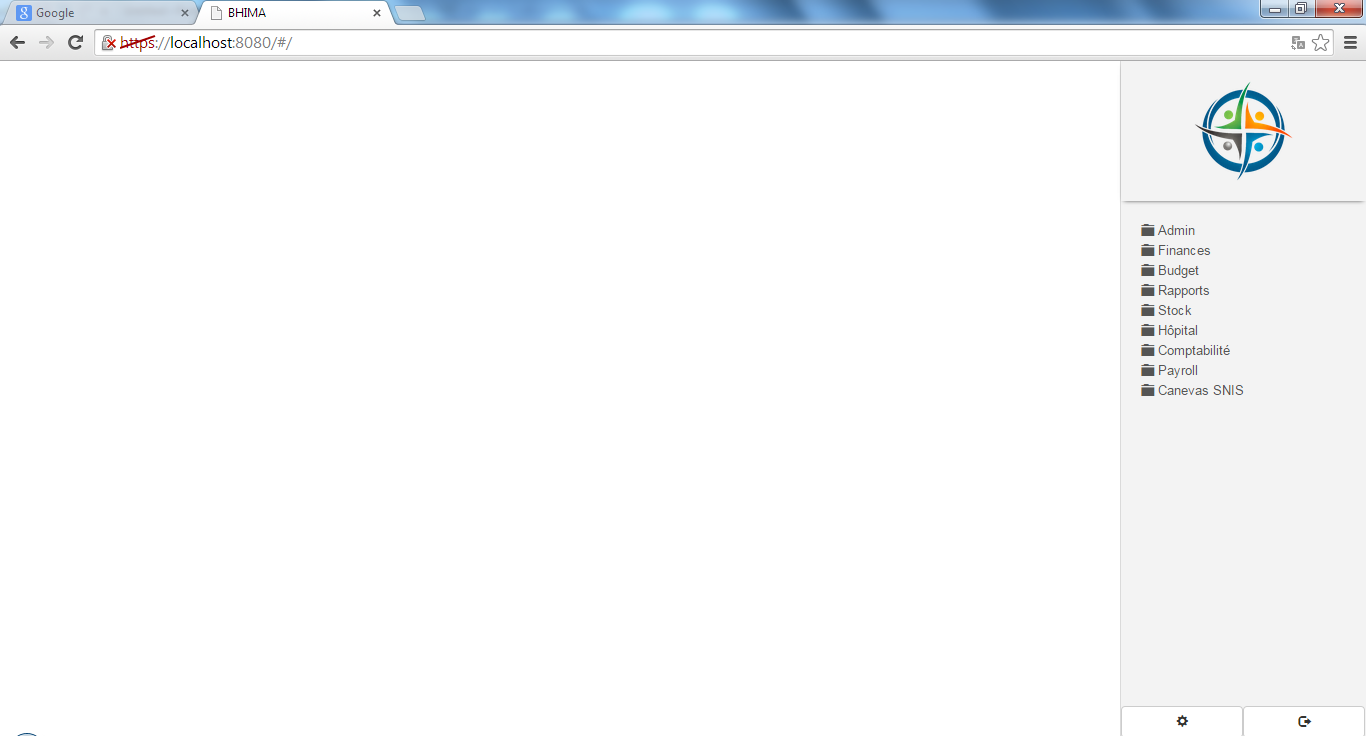
\includegraphics[width=10cm]{pic/mainInterface.png}
\end{center}
\caption{Interface principale de l'application}
\label{Interface principale de l'application}
\end{figure} 
Dans sa partie gauche de la figure ci-dessous on retrouve le logo IMA World Heath Ainsi que l'arborescence qui représente les modules du système auxquels l'utilisateur à accès. En dessous de l'arborescence figure deux boutons, le premier 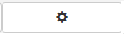
\includegraphics[scale=0.5]{pic/lang.png} permet de changer de langue et le second 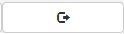
\includegraphics[scale=0.5]{pic/logout.png} permet de ce déconnecté du système.

\begin{figure}[h]
\begin{center}
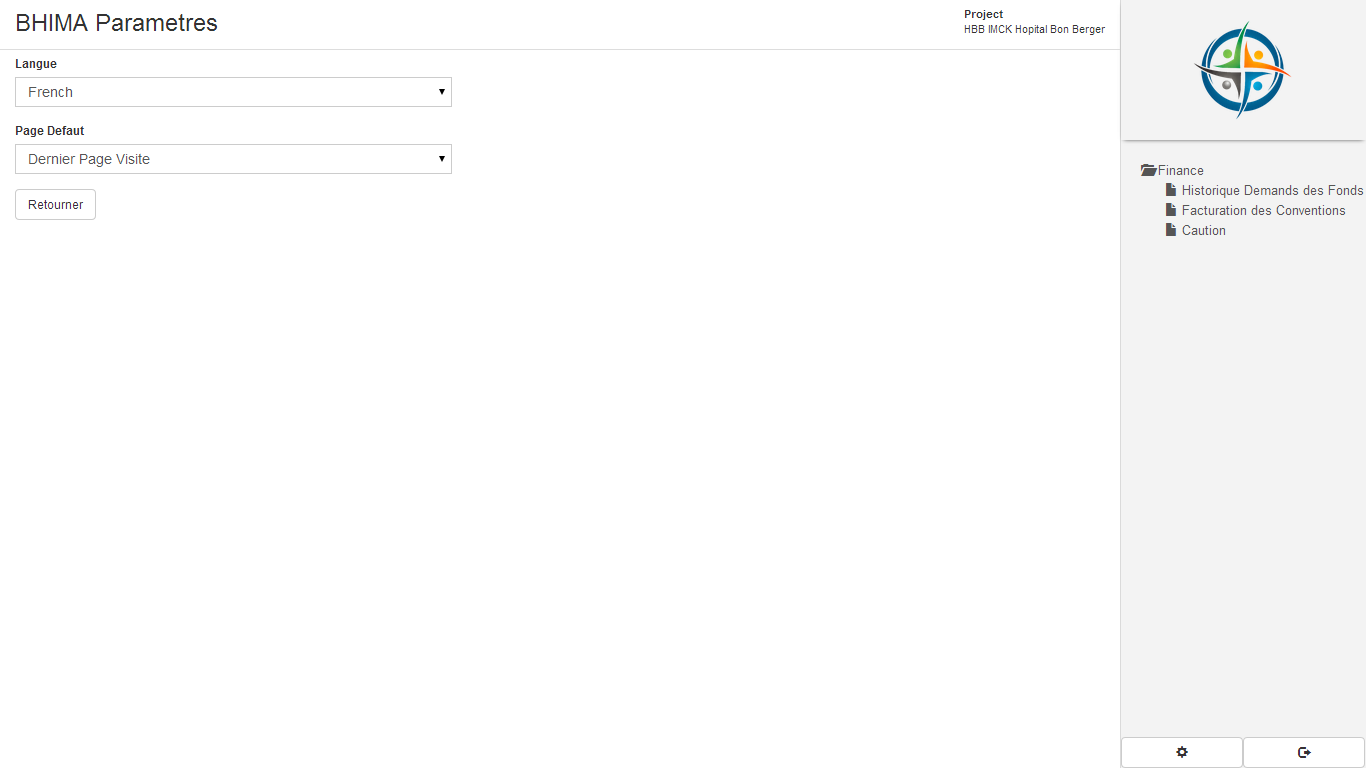
\includegraphics[width=10cm]{pic/changeLang.png}
\end{center}
\caption{Interface principale pour le changement de langue}
\label{Interface principale pour le changement de langue}
\end{figure} 

\section{Utilisation de l'arborescence de navigation}
L'arborescence de navigation contient les liens de chague module de l'application. Les modules sont regroupés en fonction de de leurs fonctionalités dans des dossiers tels que le dossier "Admin" affiché ci-dessous. Dans la première image, le dossier est fermé, en occultant tous les sous modules de ce module. Après le dossier est cliqué, une image d'un dossier ouvert montre que les contenus sont accessibles.

\begin{figure}[h]
\begin{center}
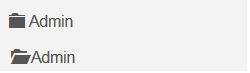
\includegraphics[width=4.5cm]{pic/folder_open_closed.png}
\end{center}
\caption{Etat d'un module ouvert et fermé}
\label{Etat d'un module ouvert et fermé}
\end{figure} 

Cliquant sur le dossier permet d'afficher la liste de sous modules sélectionné par l'utilisateur. Par exemple, ci-dessous, le dossier "Admin" est cliqué dans la premier illustration dans la séconde est ouverte tous ses sous modules.

\begin{figure}[h]
\begin{center}
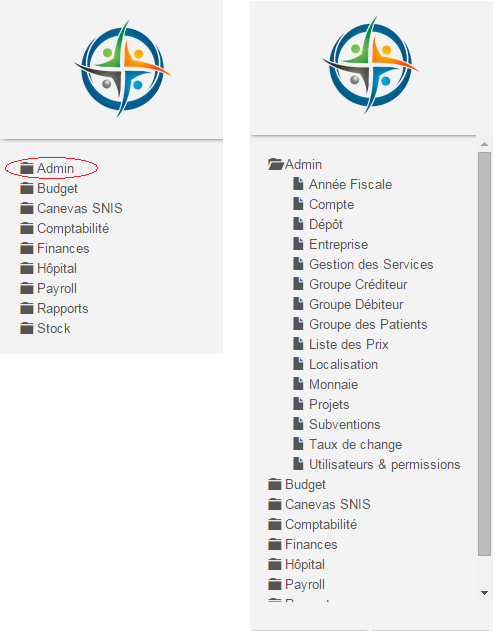
\includegraphics[width=8cm]{pic/open_folder.png}
\end{center}
\caption{Clique sur le dossier "admin" afin de pouvoir visualiser ses sous modules}
\label{Clique sur le dossier "admin" afin de pouvoir visualiser ses sous modules}
\end{figure} 


\newpage
\section{Les modules du système BHIMA}
Le système d'information BHIMA possède plusieurs modules qui sont représenté par l'arborescence ci-dessous.
\begin{figure}[h]
\begin{center}
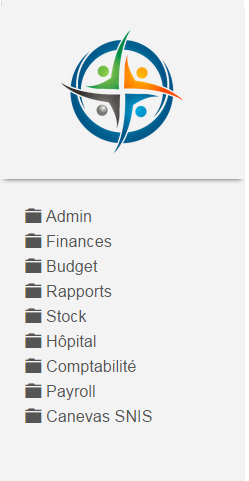
\includegraphics[width=4.5cm]{pic/arbo.png}
\end{center}
\caption{Arborescence du système}
\label{Arborescence du système}
Voici les différentes rubriques qui existent dans le système:
\end{figure} 
% Liste des modules
\begin{itemize}
\item Admin. %•
\item Budget
\item Canevas SNIS
\item Comptabilité
\item Finances
\item Hôpital
\item Payroll
\item Rapports
\item Stock
\end{itemize}


\newpage
%%%%%%%%%%%%%%%%%%%%%%%%%%%%%%%%%%%%%%%%%%%%%
%   MODULES DU SYSTEMES                     %
%%%%%%%%%%%%%%%%%%%%%%%%%%%%%%%%%%%%%%%%%%%%%

\newpage
\chapter{Le module Rapports}        
%////////////////////////////////////////////////%
Le module rapports permet de pouvoir visualiser plusieurs types des rapports résultants du fonctionnements du système, La figure ci-dessous représente avec exactitude ce module avec les différents sous éléments.

\begin{figure}[h]
\begin{center}
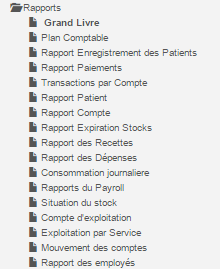
\includegraphics[width=4cm]{pic/ArboReport.png}
\end{center}
\caption{Arborescence du module Rapports}
\label{Arborescence du module Rapports}
\end{figure}

\newpage

\newpage
\section{Rapport des employés}
Le rapport des Rapport des employés permet de visualiser l'état financier d'un employé. son interface principale se présente de la manière suivante. 

\begin{figure}[h]
\begin{center}
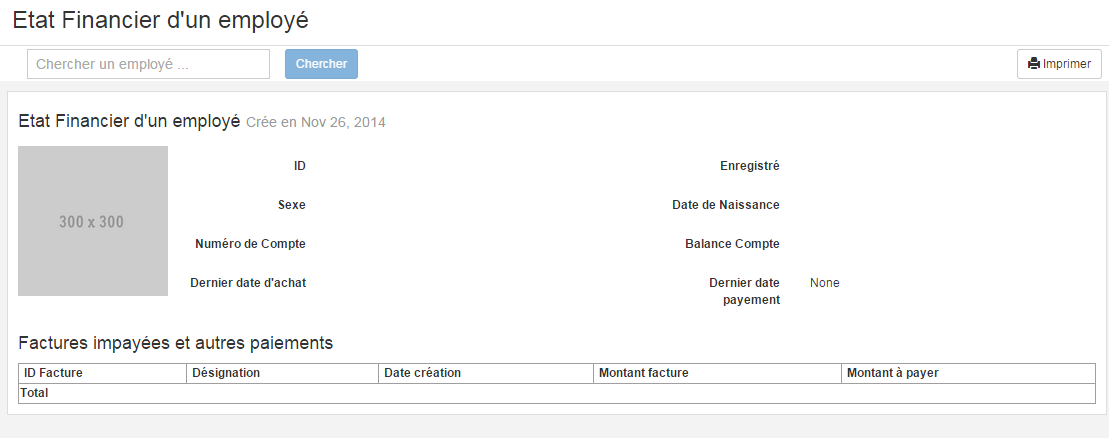
\includegraphics[width=10cm]{pic/EtFinEMp.png}
\end{center}
\caption{Aperçue de l'interface principale de l'état financier d'un employé}
\label{Aperçue de l'interface principale de l'état financier d'un employé}
\end{figure}

Le formulaire possède une zone qui permet la recherche d'un employé dans la liste des employés enregistrés, le bouton générer permet l'affichage du tableau du rapport des employés. L'interface permettant de visualier le rapport se présente de la manière suivante. Au dessus on retrouve deux boutons. le prémier 
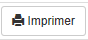
\includegraphics[scale=0.7]{pic/Print.png} permet d'imprimer le rapport et le second 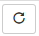
\includegraphics[scale=0.7]{pic/refresh.png} permet de faire une nouvelle recherche.

Voici un apperçue de la situation financière d'un employé.

\begin{figure}[h]
\begin{center}
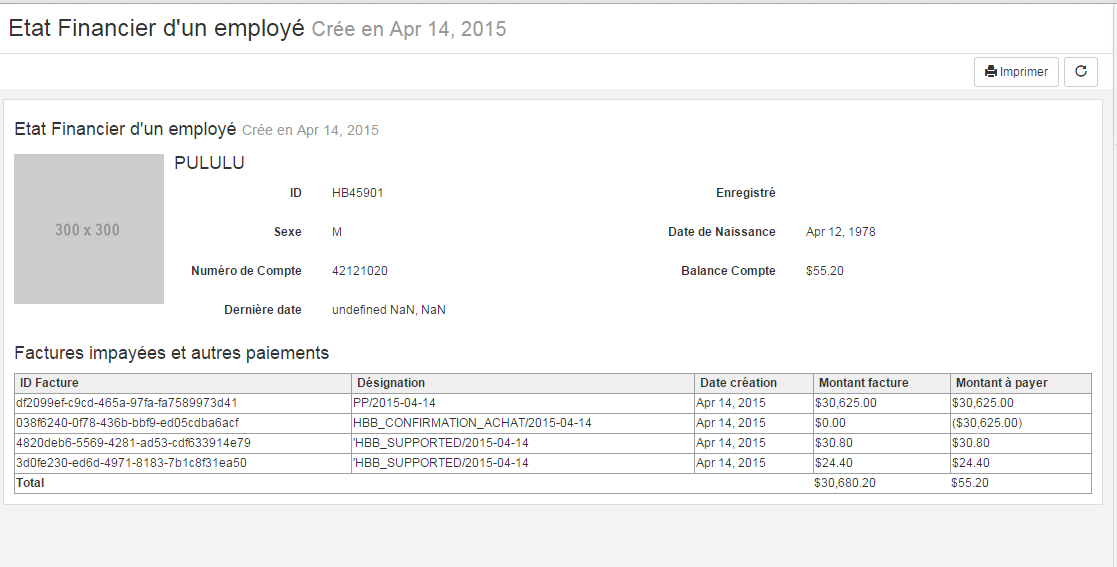
\includegraphics[width=14cm]{pic/EtFinancierEmployer.png}
\end{center}
\caption{Aperçue du rapport financier d'un employé}
\label{Aperçue du rapport financier d'un employé}
\end{figure}



\newpage
\chapter{Payroll}        
%////////////////////////////////////////////////%
Le module Payroll est composé des sous modules qui permettent d'administrer tous les éléments prises en comptes lors du processus de Payroll (Paie des employés.

\begin{figure}[h]
\begin{center}
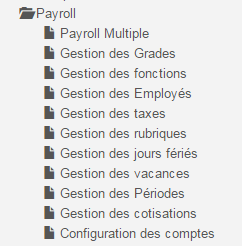
\includegraphics[width=6cm]{pic/PayrollArbo.png}
\end{center}
\caption{Arborescence du module Payroll}
\label{Arborescence du module Payroll}
\end{figure}

\newpage
\section{Payroll Multiple}
Le modules Payroll Multiple est l'interface principale qui permet d'initialiser un paiement pour une période bien déterminée.
première il faudrai sélectionner une période de paiement dans la liste de période de paiement

\begin{figure}[h]
\begin{center}
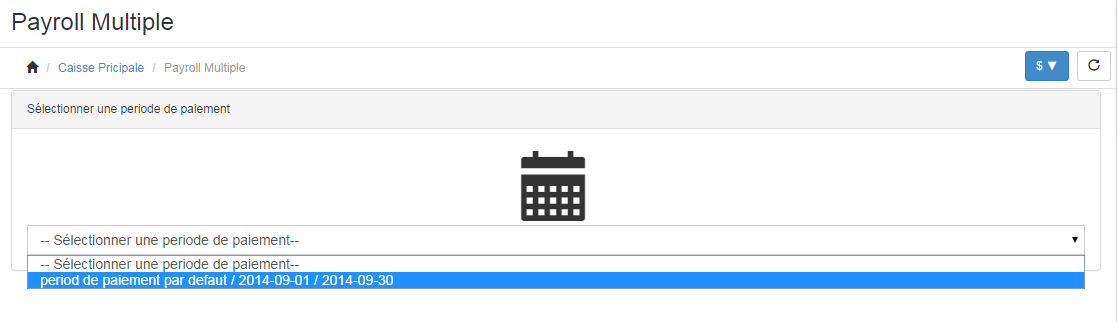
\includegraphics[width=14cm]{pic/MultiPayroll.png}
\end{center}
\caption{Interface principale du module payroll Multiple}
\label{Interface principale du module payroll Multiple}
\end{figure}
\newpage
Une fois qu'une periode de paiement est choisi, l'utilisateur est alors dirigé vers une interface possèdant l'identité de tous les employés et à la fin d'un bouton \textbf{Soumettre} qui permet de valider les processus de paiement de tous les employés à la fois, le bouton 
\includegraphics[scale=0.7]{pic/selectCurrency.png} qui permet de préciser la monnaie qui sera prise en charge lors du paiement et le bouton 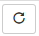
\includegraphics[scale=0.7]{pic/refresh.png} permet de réinitialiser le processus de paiement.

\begin{figure}[h]
\begin{center}
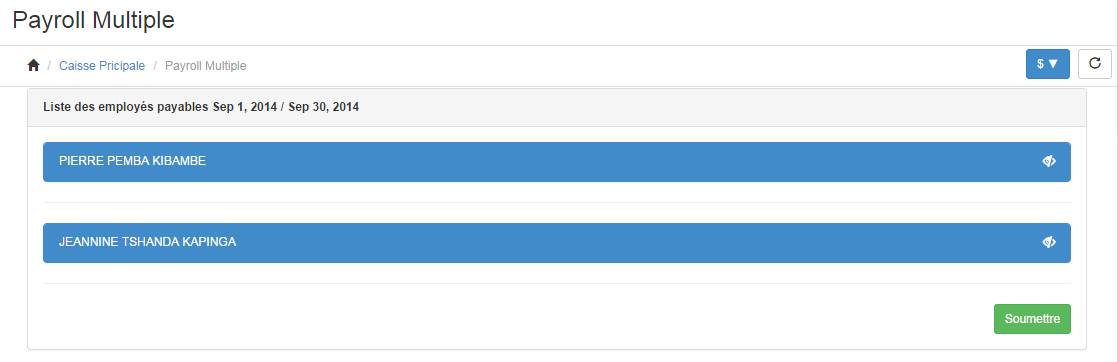
\includegraphics[width=14cm]{pic/PayrollListeEmp.png}
\end{center}
\caption{Liste des employés des employés payables durant une période de paiement}
\label{Liste des employés des employés payables durant une période de paiement}
\end{figure}

Le système permet de calculer automatiquement les nombres de jours fériés ansi que les nombres total des jours des vacances qu'un employer a obtenu au cours d'une période de paiement et précise aussi automatiquement le nombre de jour de travaille maximale pour chaque employé, s'il on veux modifier les parametres par défaut pour un employé, il suffit de cliquer sur la barre contenant son identité. Certains éléments de cette interface sont éditables et d'autres non.


\begin{figure}[h]
\begin{center}
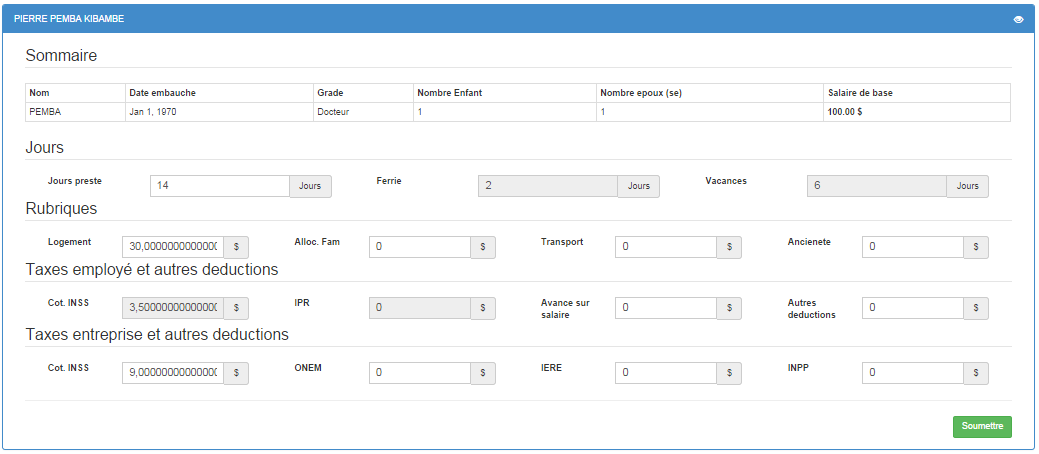
\includegraphics[width=14cm]{pic/payrollEmp.png}
\end{center}
\caption{Interface principale permettant de modifier les différents composant de la paie}
\label{Interface principale permettant de modifier les différents composant de la paie}
\end{figure}

On peut encore signaler qu'il existe un autre bouton \textbf{Soumettre} dans l'interface réservée à la modification des composants de la paie d'un employé, ce dernier permet de valider le paiement de l'employé choisi, en tenant compte de la monnaie qui est sélectionnée. 

\newpage
\section{Gestions des Grades}
Le module Gestions des grades des employés permet l'administrations des différents types des grades des employés existant au sein de l'organisation.
\begin{figure}[h]
\begin{center}
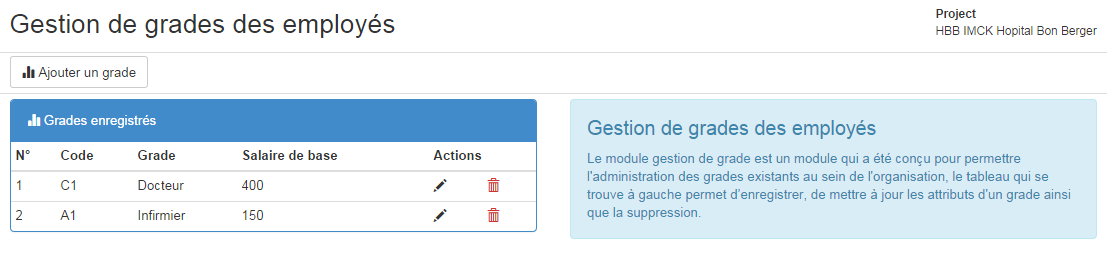
\includegraphics[width=14cm]{pic/gradeEmp.png}
\end{center}
\caption{Interface principale de la gestion des grades}
\label{Interface principale de la gestion des grades}
\end{figure}

Dans la figure ci-haute on retrouve dans la partie gauche la liste des différents grades enregistrés dans le système, au dessus de ce tableau existe le bouton 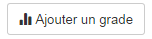
\includegraphics[scale=1]{pic/AddGrade.png} qui permet d'ajouter un nouveau grade dans le système, le formulaire permettant d'enregistrer un nouveau grade se présente de la manière suivante.

\begin{figure}[h]
\begin{center}
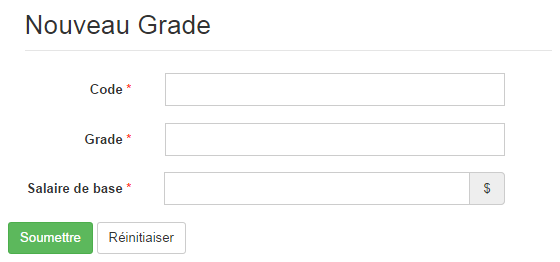
\includegraphics[width=8cm]{pic/NewGrade.png}
\end{center}
\caption{Formulaire permettant l'enregistrement des grades}
\label{Formulaire permettant l'enregistrement des grades}
\end{figure} 

Le formulaire permettant l'enregistrement des grades comporte trois zones de saisie rélative à la codification du grade au sein de l'organisation, la désignation du grade ainsi que le salaire de base par rapport à la monnaie de l'entreprise. 

\newpage
Les tableaux réprésentant les grades enregistrés donne la possibilité de pouvoir mettre à jour les informations rélative à un grade, dans la zone action de ce tableau on retrouve deux icônes, l'icône 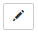
\includegraphics[scale=0.7]{pic/EditBlack.png} qui permet de mettre à jour un grade et 
\includegraphics[scale=0.7]{pic/DeleteWRed.png} permet de supprimer une grade dans le système.
Voici un apperçu du formulaire permettant la mise à jour des informations d'un grade, la mise à jour est effective que si l'on modifier les informations dont on a besoin en validant grace au bouton soumettre. 

\begin{figure}[h]
\begin{center}
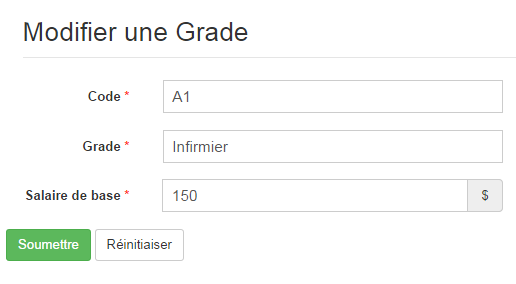
\includegraphics[width=8cm]{pic/UpdGrade.png}
\end{center}
\caption{Formulaire permettant de mettre à jour les informations d'un grade}
\label{Formulaire permettant de mettre à jour les informations d'un grade}
\end{figure} 

\newpage
\section{Gestions des fonctions}
Le module gestion de fonction est un module qui a été conçu pour permettre l'administration des fonctions existantes au sein de l'organisation, le tableau qui se trouve à gauche permet d’enregistrer, de mettre à jour les attributs d'une fonction ainsi que la suppression.
\begin{figure}[h]
\begin{center}
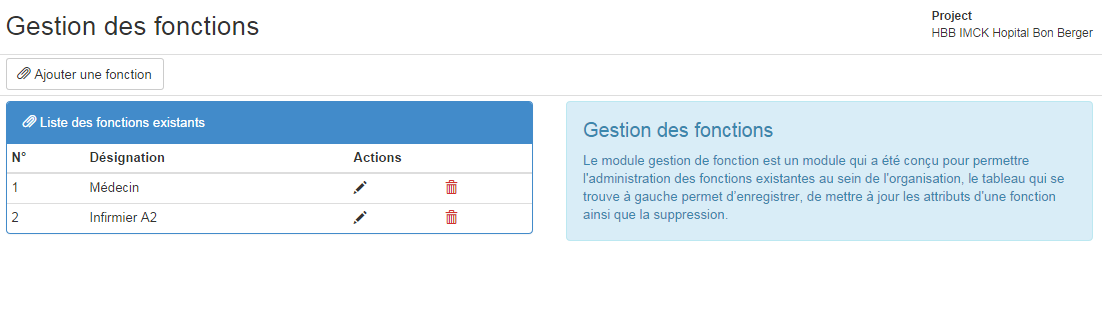
\includegraphics[width=14cm]{pic/GestionFonction.png}
\end{center}
\caption{Interface principale de la gestion des fonctions}
\label{Interface principale de la gestion des fonctions}
\end{figure}

Dans la figure ci-haute on retrouve dans la partie gauche la liste des différents fonctions enregistrées dans le système, au dessus de ce tableau existe le bouton 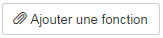
\includegraphics[scale=1]{pic/AddFonction.png} qui permet d'ajouter une nouvelle fonction dans le système, le formulaire permettant d'enregistrer une nouvelle fonction se présente de la manière suivante.

\begin{figure}[h]
\begin{center}
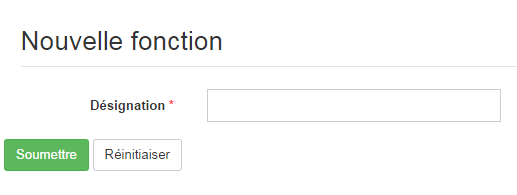
\includegraphics[width=8cm]{pic/FormAddFonction.png}
\end{center}
\caption{Formulaire permettant l'enregistrement des fonctions}
\label{Formulaire permettant l'enregistrement des fonctions}
\end{figure} 

Le formulaire permettant l'enregistrement des fonctions est très simple, il ne contient que la zone de saisie permettant de renseigner la designation de la fonction, et l'enregistrement est effective que si l'on clique sur le bouton soumettre. 

\newpage
Les tableaux réprésentant les fonctions enregistrées donne la possibilité de pouvoir mettre à jour les informations rélative à une fonction, dans la zone action de ce tableau on retrouve deux icônes, l'icône 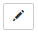
\includegraphics[scale=0.7]{pic/EditBlack.png} qui permet de mettre à jour une fonction et 
\includegraphics[scale=0.7]{pic/DeleteWRed.png} permet de supprimer une fonction dans le système.
Voici un apperçu du formulaire permettant la mise à jour des informations d'un fonction, la mise à jour est effective que si l'on modifier les informations dont on a besoin en validant grace au bouton soumettre. 

\begin{figure}[h]
\begin{center}
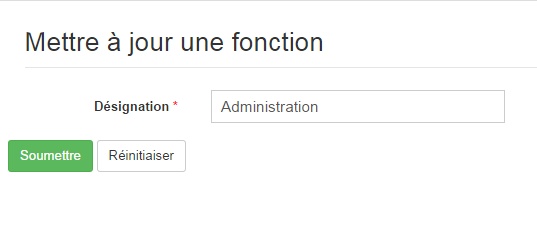
\includegraphics[width=8cm]{pic/MettreAJFonction.png}
\end{center}
\caption{Formulaire permettant de mettre à jour une fonction}
\label{Formulaire permettant de mettre à jour une fonction}
\end{figure} 


\newpage
\section{Gestions des employés}
Ce menu permet d'enregistré les employés travaillant au sein de l'entreprise, mais aussi de modifier leur informations rélatives, ainsi que leur différentes 	attributions, l'interface principale de ce modules se présente de la manière suivante.


\begin{figure}[h]
\begin{center}
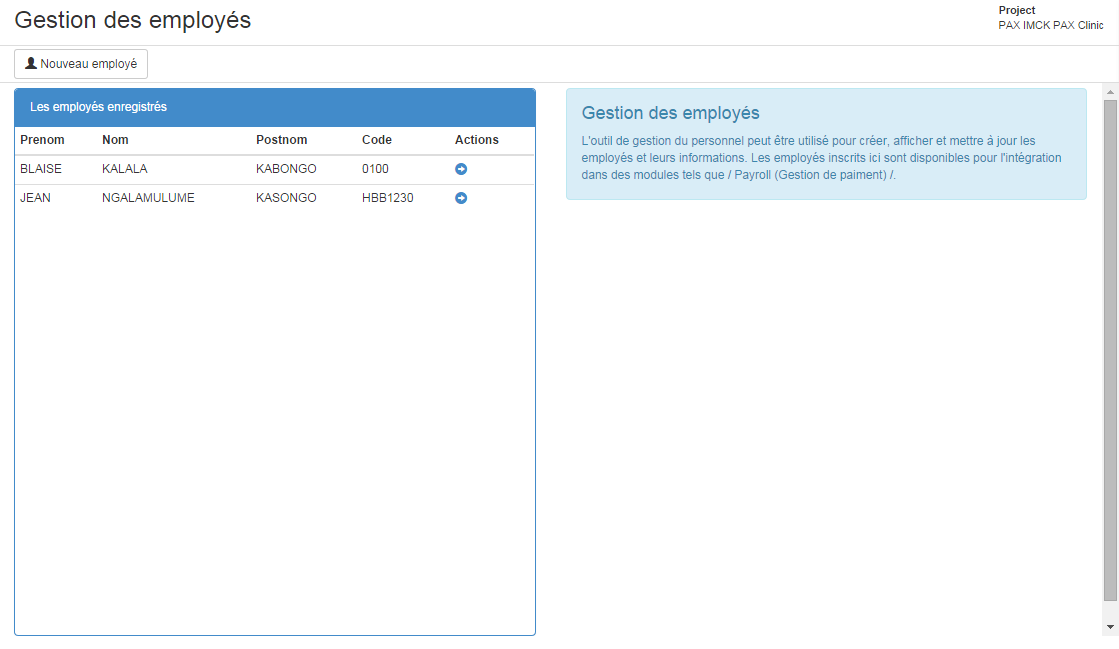
\includegraphics[width=14cm]{pic/AdminEmp.png}
\end{center}
\caption{Interface principale de la gestion des employés}
\label{Interface principale de la gestion des employés}
\end{figure}

Dans la figure ci-haut on retrouve dans la partie gauche la liste des employés enregistrés dans le système, au dessus de ce tableau il existe le bouton 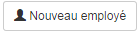
\includegraphics[scale=1]{pic/New_emp.png} qui permet d'ajouter un nouveau employé dans le système, le formulaire permettant d'enregistrer un nouveau employé se présente de la manière suivante.

\begin{figure}[h]
\begin{center}
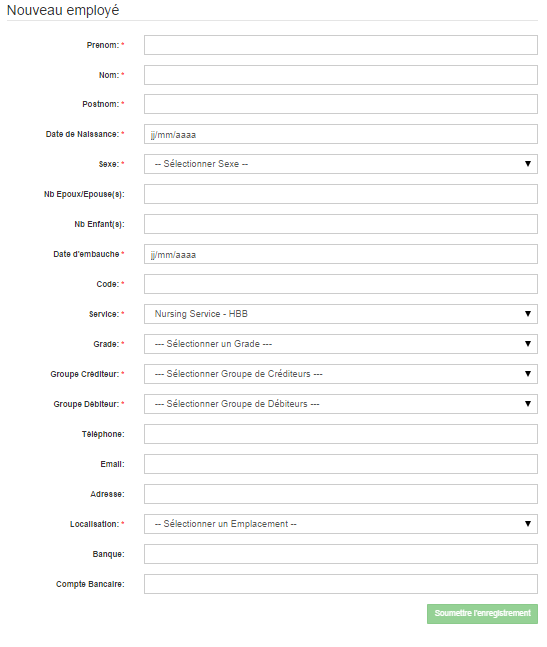
\includegraphics[width=8cm]{pic/FormNewEmp.png}
\end{center}
\caption{Formulaire permettant l'enregistrement des employés}
\label{Formulaire permettant l'enregistrement des employés}
\end{figure} 


L'enregistrement n'est possible que si tous les champs obliqatoires sont renseignés et si l'on valide l'enregistrement en cliquant sur le bouton Soumettre l'enregistrement. 

Les tableaux réprésentant les employés enregistrés donne la possibilité de pouvoir mettre à jour les informations rélative à un employés, ce tableau comporte 5 rubriques: Prenom, Nom, Postnom, Code ainsi que la zone réservée à la modification, cette zone possède l'icône 
\includegraphics[scale=0.7]{pic/PlusUpdate.png}, qui permet de modifier le méta donné d'un employés, si l'on clique sur ce dernier le formulaire s'affiche dans la partie droite de l'ecran avec les informations rélatives à un employés avec la possibilité de modifier si nécessaire et à valider les modifications grace au bouton Envoyer les détails.


\newpage
\section{Gestion des Taxes}
Le module gestions des taxes permet l'administration des différents types des taxes existant au sein de l'entreprise lors du paiement des employés. Son interface principale est constituée d'un menu qui permet la création d'une taxe, la configuration du taxe IPR ainsi que la configuration des taxes qui seront prise en compte lors du paiement des agents.
\begin{figure}[h]
\begin{center}
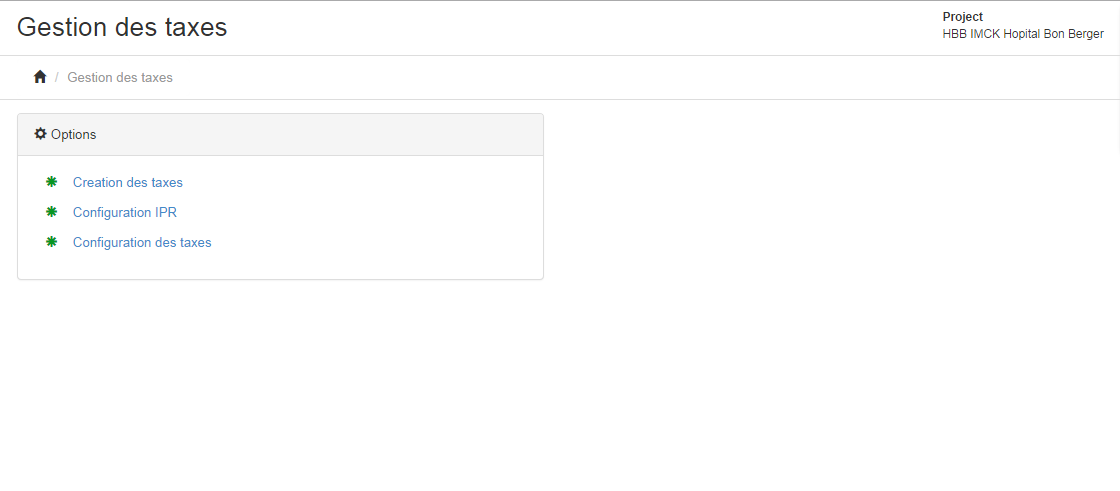
\includegraphics[width=14cm]{pic/GesTaxes.png}
\end{center}
\caption{Interface principale du module gestion des Taxes}
\label{Interface principale du module gestion des Taxes}
\end{figure}

\newpage
\subsection{Création des Taxes}
Le module création de taxes est un module qui a été conçu pour permettre l'administration des taxes existants au sein de l'organisation,
\begin{figure}[h]
\begin{center}
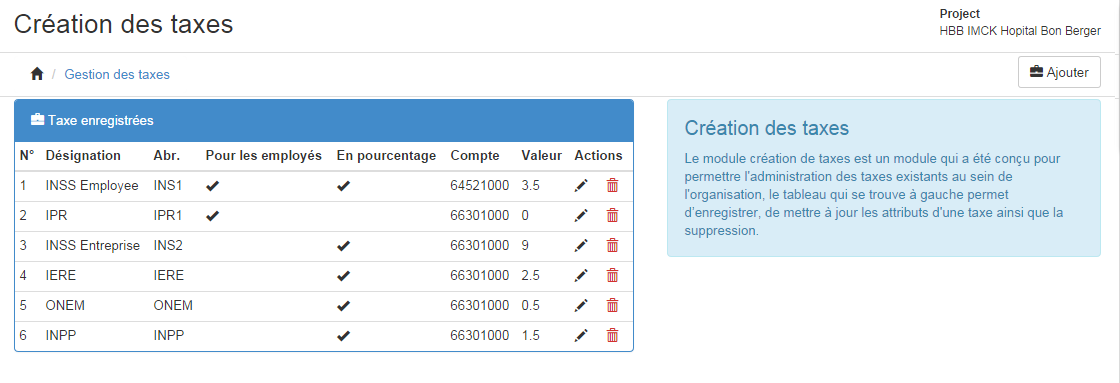
\includegraphics[width=14cm]{pic/GesCreaTaxes.png}
\end{center}
\caption{Interface principale de la création des taxes}
\label{Interface principale de la création des taxes}
\end{figure}

Dans la figure ci-haute on retrouve une barre de navigation permettant de rentrer vers le menu principale sur la gestion des taxes, à droite de la barre de navigation il existe le bouton 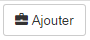
\includegraphics[scale=1]{pic/AddTaxe.png} qui permet d'ajouter une nouvelle taxe, il existe également en dessous de la barre de navigation dans la partie gauche le tableau des taxes enregistrées.

Le formulaire permettant d'ajouter une taxe se présente de la manière suivante. 

\begin{figure}[h]
\begin{center}
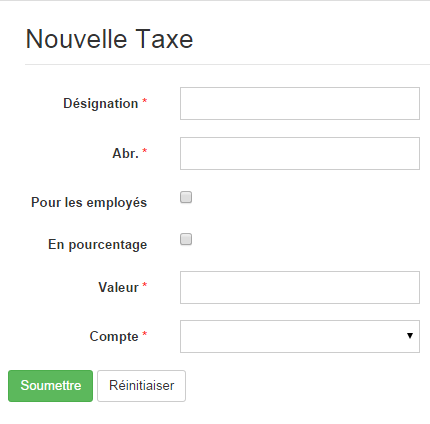
\includegraphics[width=8cm]{pic/NouvTaxe.png}
\end{center}
\caption{Formulaire permettant d'ajouter une taxe}
\label{Formulaire permettant d'ajouter une taxe}
\end{figure} 

Pour l'enregistrement d'une taxe les informations suivantes doivent être fourni, la désignation de la taxe, son abbréviation avec aux maximum quatre lettres, spécifier si cette taxe est payable par l'employé si non elle est par l'entreprise, spécifier aussi si elle s'exprime en pourcentage mais aussi la valeur de ce pourcentage, si elle ne s'exprime pas en pourcentage dans ce cas la zone de saisie \textbf{Valeur} exprime alors le montant par rapport à la monnaie principale de l'entreprise équivalent à la taxe et en dernier il faudrait spécifier le compte équivalent au paiement de la dite taxe. 

Les tableaux réprésentant les taxes enregistrées donne la possibilité de pouvoir mettre à jour les informations rélative à une taxe, dans la zone action de ce tableau on retrouve deux icônes, l'icône 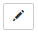
\includegraphics[scale=0.7]{pic/EditBlack.png} qui permet de mettre à jour une taxe et 
\includegraphics[scale=0.7]{pic/DeleteWRed.png} permet de supprimer une taxe dans le système.
Voici un apperçu du formulaire permettant la mise à jour des informations d'une taxe, la mise à jour est effective que si l'on modifier les informations dont on a besoin en validant grace au bouton soumettre. 

\begin{figure}[h]
\begin{center}
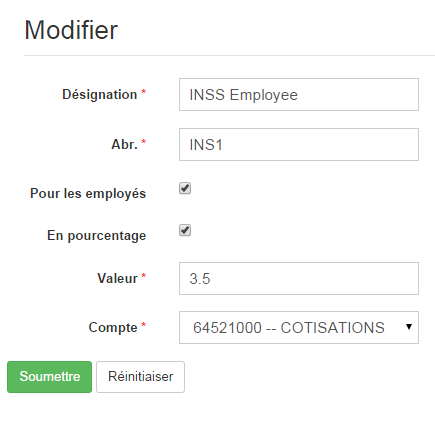
\includegraphics[width=8cm]{pic/ModTaxe.png}
\end{center}
\caption{Formulaire permettant de mettre à jour les informations d'une taxe}
\label{Formulaire permettant de mettre à jour les informations d'une taxe}
\end{figure} 
\newpage
\subsection{Configuration de la taxe IPR}
Le module configuration de la taxe IPR est un modile qui a été conçu pour permettre l'administration des différentes taches utilisés lors du calcul de la tranche IPR. 
\begin{figure}[h]
\begin{center}
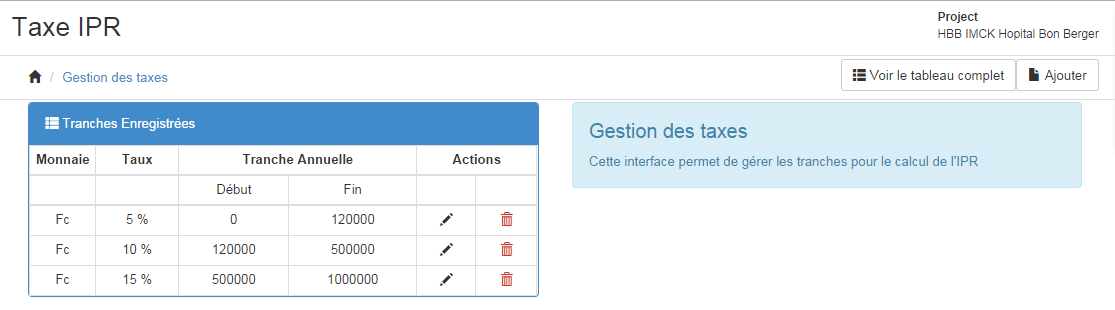
\includegraphics[width=14cm]{pic/TaxeIPR.png}
\end{center}
\caption{Interface principale de la configuration du taxe IPR}
\label{Interface principale de la configuration du taxe IPR}
\end{figure}

Dans la figure ci-haute on retrouve une barre de navigation permettant de rentrer vers le menu principale sur la gestion des taxes, à droite de la barre de navigation il existe deux bouton, le bouton 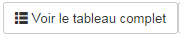
\includegraphics[scale=1]{pic/TabComplet.png} qui permet de visualier les tranches de l'IPR configurées et le bouton 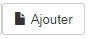
\includegraphics[scale=1]{pic/AddIPR.png} permet d'ajouter une nouvelle tranche dans la configuration, il existe également en dessous de la barre de navigation dans la partie gauche le tableau des différentes tranches enregistrées.

Le formulaire permettant la configuration d'une nouvelle tranche se présente de la manière suivante. 

\begin{figure}[h]
\begin{center}
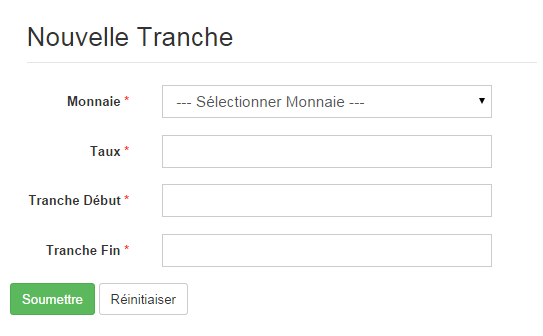
\includegraphics[width=8cm]{pic/NouvTranche.png}
\end{center}
\caption{Formulaire permettant la configuration d'une tranche}
\label{Formulaire permettant la configuration d'une tranche}
\end{figure} 


Pour la configuration d'une taxe les informations suivantes doivent être fourni, premièrement la monnaie utilisé lors de la configuration de l'IPR et une fois qu'une monnaie est utilisée elle restera la monnaie par défaut lors de toute opération des configurations, le taux désigne le pourcentage correspondant à la dite tranche et tranche début et tranche fin correspond à la plage de valeur annuelle  délimitant une plage. 

Les tableaux réprésentant les tranches enregistrées donne la possibilité de pouvoir mettre à jour les informations rélative à une tranche, dans la zone action de ce tableau on retrouve deux icônes, l'icône 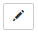
\includegraphics[scale=0.7]{pic/EditBlack.png} qui permet de mettre à jour les informations rélatives à une tranche et 
\includegraphics[scale=0.7]{pic/DeleteWRed.png} permet de supprimer une tranche.
Voici un apperçu du formulaire permettant la mise à d'une tranche, la mise à jour est effective que si l'on modifier les informations dont on a besoin en validant grace au bouton soumettre. 

\begin{figure}[h]
\begin{center}
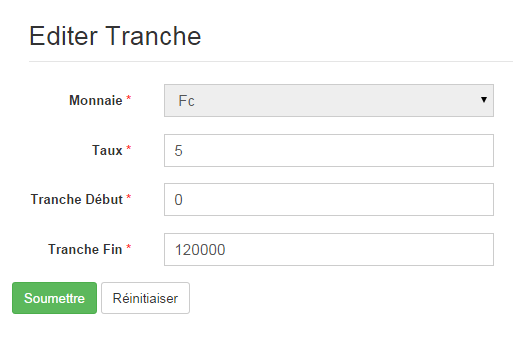
\includegraphics[width=8cm]{pic/EditTranche.png}
\end{center}
\caption{Formulaire permettant de mettre à jour les informations d'une tranche}
\label{Formulaire permettant de mettre à jour les informations d'une tranche}
\end{figure}

Voici un apperçue des différents tranches utilisés lors du calcul de l'IPR, le bouton \textbf{changer de vue} permet de revenir dans la page principale de la configuration du taxe IPR.

\begin{figure}[h]
\begin{center}
\includegraphics[width=15cm]{pic/ConfigTaxes.png}
\end{center}
\caption{Apperçue global des tranches IPR configurées}
\label{Apperçue global des tranches IPR configurées}
\end{figure}

\newpage
\subsection{Configuration des taxes}
Le module configuration des taxes, permet le paramétrage des différentes types taxes qui sont prises pendant une période de paie.

\begin{figure}[h]
\begin{center}
\includegraphics[width=14cm]{pic/ConfTaxePeriod.png}
\end{center}
\caption{Interface principale de la configuration des taxes}
\label{Interface principale de la configuration des taxes}
\end{figure}

Dans la figure ci-haute on retrouve une barre de navigation permettant de rentrer vers le menu principale sur la gestion des taxes, à droite de la barre de navigation il existe le bouton \includegraphics[scale=1]{pic/CreateNewConfig.png} qui permet d'ajouter une nouvelle configuration de taxe, il existe également en dessous de la barre de navigation dans la partie gauche le tableau des configurations de taxes enregistrées.

Le formulaire permettant l'ajout d'une nouvelle configuration se présente de la manière suivante. 

\begin{figure}[h]
\begin{center}
\includegraphics[width=8cm]{pic/NouvConfigT.png}
\end{center}
\caption{Formulaire permettant la création d'une nouvelle configuration}
\label{Formulaire permettant la création d'une nouvelle configuration}
\end{figure} 

\newpage
Pour l'enregistrement d'une nouvelle configuration, il suffit de fournir la designation d'une nouvelle configuration ensuite de cliquer sur le bouton \textbf{Soumettre}.
\\

Les tableaux réprésentant les configurations enregistrées donne la possibilité de pouvoir mettre à jour les informations rélative à une configuration, dans la zone action de ce tableau on retrouve trois icônes, l'icône \includegraphics[scale=0.7]{pic/EditUser.png} qui permet de mettre à jour la désignation de la configuration, l'icône  \includegraphics[scale=0.7]{pic/PlusConfigBlue.png} qui permet de faire la configuration proprement dite et  et l'icône  \includegraphics[scale=0.7]{pic/DeleteWRed.png} permet de supprimer une configuration dans le système.
Le formulaire permettant la mise à jour des informations d'une configurations est très simple et ne possède que la zone de saisie permettant la modification de la designation ainsi que le bouton \textbf{Soumettre} pour confirmer la mise à jour.

\begin{figure}[h]
\begin{center}
\includegraphics[width=8cm]{pic/UpDConfgTax.png}
\end{center}
\caption{Formulaire permettant de mettre à la designation d'une configuration}
\label{Formulaire permettant de mettre à la designation d'une configuration}
\end{figure} 

Le bouton  \includegraphics[scale=0.7]{pic/PlusConfigBlue.png} permet d'accomplire la configuration proprement dite, l'interface de configuration se présente de la manière suivante.  
\begin{figure}[h]
\begin{center}
\includegraphics[width=8cm]{pic/ConfigTaxesMenu.png}
\end{center}
\caption{Formulaire permettant de mettre à la designation d'une configuration}
\label{Formulaire permettant de mettre à la designation d'une configuration}
\end{figure} 

Dans l'image ci-haute, est repris le nom de la configuration dont on veut paramettrer ainsi que la liste de différente taxe qui existe dans le système, ces différentes taxes possèdes des cases à cocher qui permet de préciser les différentes taxes qui fairons partie de la dite configuration, il est aussi possible de sélectionner toutes les taxes en une seule fois simplement en cochant l'option tous, et une fois qu'on coché les taxes qui feront parties de la configuration le bouton \includegraphics[scale=0.7]{pic/SaveConfig.png} permet d'enregistrer la configuration, en plus ce même bouton permet aussi de faire la mise à jour des taxes faisant partie d'une configuration.

\newpage
\section{Gestion des Rubriques}
Le module gestions des rubriques permet l'administration des différents types des rubriques existant au sein de l'entreprise lors du paiement des employés. Son interface principale est constituée d'un menu qui permet l'ajout des rubriques payroll ainsi que la configuration des rubriques qui seront prise en compte lors du paiement des agents.
\begin{figure}[h]
\begin{center}
\includegraphics[width=14cm]{pic/GestRubriques.png}
\end{center}
\caption{Interface principale du module gestion des Rubriques}
\label{Interface principale du module gestion des Rubriques}
\end{figure}

\subsection{Rubriques Payroll}
Le module Rubriques Payroll est un module qui a été conçu pour permettre l'administration des différents rubriques existants au sein de l'organisation,
\begin{figure}[h]
\begin{center}
\includegraphics[width=14cm]{pic/RubPayroll.png}
\end{center}
\caption{Interface principale de la création des rubriques}
\label{Interface principale de la création des rubriques}
\end{figure}

Dans la figure ci-haute on retrouve une barre de navigation permettant de rentrer vers le menu principale sur la gestion des rubriques, à droite de la barre de navigation il existe le bouton \includegraphics[scale=1]{pic/AddRubriques.png} qui permet d'ajouter une nouvelle rubrique, il existe également en dessous de la barre de navigation dans la partie gauche le tableau des rubriques enregistrées.

Le formulaire permettant d'ajouter une rubrique se présente de la manière suivante. 

\begin{figure}[h]
\begin{center}
\includegraphics[width=8cm]{pic/NewRubric.png}
\end{center}
\caption{Formulaire permettant d'ajouter une rubrique}
\label{Formulaire permettant d'ajouter une rubrique}
\end{figure} 

Pour l'enregistrement d'une rubrique les informations suivantes doivent être fourni, la désignation de la rubrique, son abbréviation avec aux maximum quatre lettres, spécifier si cette rubrique s'exprime en pourcentage, spécifier si cette rubrique est une charge pour l'employé ou bien un gain ainsi que la valeur de ce pourcentage, si elle ne s'exprime pas en pourcentage dans ce cas la zone de saisie \textbf{Valeur} exprime alors le montant par rapport à la monnaie principale de l'entreprise équivalent à la rubrique, spécifier aussi si cette rubrique fait partie des charges sociales (n'intervenant que dans le net après taxe), il est aussi possible de pouvoir distingué la rubrique (Avance sur salaire pour retenir automatique le montant du salaire avancé). 

Les tableaux réprésentant les rubriques enregistrées donne la possibilité de pouvoir mettre à jour les informations rélative à une rubriques, dans la zone action de ce tableau on retrouve deux icônes, l'icône \includegraphics[scale=0.7]{pic/EditBlack.png} qui permet de mettre à jour une rubrique et \includegraphics[scale=0.7]{pic/DeleteWRed.png} permet de supprimer une rubriques dans le système.
Voici un apperçu du formulaire permettant la mise à jour des informations d'une rubrique, la mise à jour est effective que si l'on modifier les informations dont on a besoin en validant grace au bouton soumettre. 
\newpage
\begin{figure}[h]
\begin{center}
\includegraphics[width=8cm]{pic/EditRubrique.png}
\end{center}
\caption{Formulaire permettant de mettre à jour les informations d'une rubrique}
\label{Formulaire permettant de mettre à jour les informations d'une rubrique}
\end{figure} 

\newpage
\subsection{Configuration des Rubriques}
Le module configuration des rubriques, permet le paramétrage des différentes types rubriques qui sont prises pendant une période de paie.

\begin{figure}[h]
\begin{center}
\includegraphics[width=14cm]{pic/ConfigRubriques.png}
\end{center}
\caption{Interface principale de la configuration des rubriques}
\label{Interface principale de la configuration des rubriques}
\end{figure}

Dans la figure ci-haute on retrouve une barre de navigation permettant de rentrer vers le menu principale sur la gestion des rubriques, à droite de la barre de navigation il existe le bouton \includegraphics[scale=1]{pic/CreatNCRub.png} qui permet d'ajouter une nouvelle configuration de rubriques, il existe également en dessous de la barre de navigation dans la partie gauche le tableau des configurations des rubriques enregistrées.

Le formulaire permettant l'ajout d'une nouvelle configuration se présente de la manière suivante. 

\begin{figure}[h]
\begin{center}
\includegraphics[width=8cm]{pic/NouvConfigR.png}
\end{center}
\caption{Formulaire permettant la création d'une nouvelle configuration}
\label{Formulaire permettant la création d'une nouvelle configuration}
\end{figure} 

Pour l'enregistrement d'une nouvelle configuration, il suffit de fournir la designation d'une nouvelle configuration ensuite de cliquer sur le bouton \textbf{Soumettre}.

Les tableaux réprésentant les configurations enregistrées donne la possibilité de pouvoir mettre à jour les informations rélative à une configuration, dans la zone action de ce tableau on retrouve trois icônes, l'icône \includegraphics[scale=0.7]{pic/EditUser.png} qui permet de mettre à jour la désignation de la configuration, l'icône  \includegraphics[scale=0.7]{pic/PlusConfigBlue.png} qui permet de faire la configuration proprement dite et  et l'icône  \includegraphics[scale=0.7]{pic/DeleteWRed.png} permet de supprimer une configuration dans le système.

\newpage
Le formulaire permettant la mise à jour des informations d'une configurations est très simple et ne possède que la zone de saisie permettant la modification de la designation ainsi que le bouton \textbf{Soumettre} pour confirmer la mise à jour.

\begin{figure}[h]
\begin{center}
\includegraphics[width=8cm]{pic/UpDConfgRub.png}
\end{center}
\caption{Formulaire permettant de mettre à la designation d'une configuration}
\label{Formulaire permettant de mettre à la designation d'une configuration}
\end{figure} 

\newpage
Le bouton  \includegraphics[scale=0.7]{pic/PlusConfigBlue.png} permet d'accomplire la configuration proprement dite, l'interface de configuration se présente de la manière suivante.  
\begin{figure}[h]
\begin{center}
\includegraphics[width=8cm]{pic/ConfigRubMenu.png}
\end{center}
\caption{Formulaire permettant la configuration}
\label{Formulaire permettant la configuration}
\end{figure} 

Dans l'image ci-haute, est repris le nom de la configuration dont on veut paramettrer ainsi que la liste des différentes rubriques qui existent dans le système, ces différentes rubriques possèdes des cases à cocher qui permet de préciser les différentes rubriques qui fairons partie de la dite configuration, il est aussi possible de sélectionner toutes les taxes en une seule fois simplement en cochant l'option tous, et une fois qu'on coché les rubriques qui feront parties de la configuration le bouton \includegraphics[scale=0.7]{pic/SaveConfig.png} permet d'enregistrer la configuration, en plus ce même bouton permet aussi de faire la mise à jour des rubriques faisant partie d'une configuration.

\newpage

\section{Gestion des cotisations}
Le module Gestion des cotisations permet l'administration des différents types des cotisation existant au sein de l'entreprise lors du paiement des employés. Son interface principale est constituée d'un menu qui permet l'ajout des cotisations ainsi que la configuration des cotisations qui seront prise en compte lors du paiement des agents.
\begin{figure}[h]
\begin{center}
\includegraphics[width=14cm]{pic/MainCotisations.png}
\end{center}
\caption{Interface principale du module gestion des cotisations}
\label{Interface principale du module gestion des cotisations}
\end{figure}

\subsection{Création des cotisations}
Le module Création des cotisations est un module qui a été conçu pour permettre l'administration des cotisations existants au sein de l'organisation,

\begin{figure}[h]
\begin{center}
\includegraphics[width=14cm]{pic/CreatCotisationInterface.png}
\end{center}
\caption{Interface principale de la création des cotisations}
\label{Interface principale de la création des cotisations}
\end{figure}

Dans la figure ci-haute on retrouve une barre de navigation permettant de rentrer vers le menu principale sur la gestion des cotisations, à droite de la barre de navigation il existe le bouton \includegraphics[scale=1]{pic/AjouterCotisation.png} qui permet d'ajouter une nouvelle cotisation, il existe également en dessous de la barre de navigation dans la partie gauche le tableau des cotisations déjà enregistrées.

Le formulaire permettant d'ajouter une nouvelle cotisations se présente de la manière suivante. 

\begin{figure}[h]
\begin{center}
\includegraphics[width=8cm]{pic/NewCotisationForm.png}
\end{center}
\caption{Formulaire permettant d'ajouter une cotisation}
\label{Formulaire permettant d'ajouter une cotisation}
\end{figure} 

Pour l'enregistrement d'une cotisation les informations suivantes doivent être fourni, la désignation de la cotisation, son abbréviation avec aux maximum quatre lettres, spécifier si cette cotisation s'exprime en pourcentage, si elle ne s'exprime pas en pourcentage dans ce cas la zone de saisie \textbf{Valeur} exprime alors le montant par rapport à la monnaie principale de l'entreprise équivalent à la cotisation. 

Les tableaux réprésentant les cotisationq enregistrées donne la possibilité de pouvoir mettre à jour les informations rélative à une rubriques, dans la zone action de ce tableau on retrouve deux icônes, l'icône \includegraphics[scale=0.7]{pic/EditBlack.png} qui permet de mettre à jour une cotisation et \includegraphics[scale=0.7]{pic/DeleteWRed.png} permet de supprimer une cotisation dans le système.
Voici un apperçu du formulaire permettant la mise à jour des informations d'une cotisation, la mise à jour est effective que si l'on modifier les informations dont on a besoin en validant grace au bouton soumettre. 
\newpage
\begin{figure}[h]
\begin{center}
\includegraphics[width=8cm]{pic/ModCotisations.png}
\end{center}
\caption{Formulaire permettant de mettre à jour les informations d'une cotisation}
\label{Formulaire permettant de mettre à jour les informations d'une cotisation}
\end{figure} 


\subsection{Configuration des Cotisations}
Le module configuration des cotisations, permet le paramétrage des différentes types cotisations qui sont prises pendant une période de paie.

\begin{figure}[h]
\begin{center}
\includegraphics[width=14cm]{pic/ConfigCotisation.png}
\end{center}
\caption{Interface principale de la configuration des cotisations}
\label{Interface principale de la configuration des cotisations}
\end{figure}

Dans la figure ci-haute on retrouve une barre de navigation permettant de rentrer vers le menu principale sur la gestion des cotisations, à droite de la barre de navigation il existe le bouton \includegraphics[scale=1]{pic/CreatNCRub.png} qui permet d'ajouter une nouvelle configuration de cotisation, il existe également en dessous de la barre de navigation dans la partie gauche le tableau des configurations des cotisations enregistrées.

Le formulaire permettant l'ajout d'une nouvelle configuration se présente de la manière suivante. 

\begin{figure}[h]
\begin{center}
\includegraphics[width=8cm]{pic/NouvCotisation.png}
\end{center}
\caption{Formulaire permettant la création d'une nouvelle configuration}
\label{Formulaire permettant la création d'une nouvelle configuration}
\end{figure} 

\newpage
Pour l'enregistrement d'une nouvelle configuration, il suffit de fournir la designation d'une nouvelle configuration ensuite de cliquer sur le bouton \textbf{Soumettre}.
\\

Les tableaux réprésentant les configurations enregistrées donne la possibilité de pouvoir mettre à jour les informations rélative à une configuration, dans la zone action de ce tableau on retrouve trois icônes, l'icône \includegraphics[scale=0.7]{pic/EditUser.png} qui permet de mettre à jour la désignation de la configuration, l'icône  \includegraphics[scale=0.7]{pic/PlusConfigBlue.png} qui permet de faire la configuration proprement dite et  et l'icône  \includegraphics[scale=0.7]{pic/DeleteWRed.png} permet de supprimer une configuration dans le système.
Le formulaire permettant la mise à jour des informations d'une configurations est très simple et ne possède que la zone de saisie permettant la modification de la designation ainsi que le bouton \textbf{Soumettre} pour confirmer la mise à jour.

\begin{figure}[h]
\begin{center}
\includegraphics[width=8cm]{pic/MetJCotisation.png}
\end{center}
\caption{Formulaire permettant de mettre à la designation d'une configuration}
\label{Formulaire permettant de mettre à la designation d'une configuration}
\end{figure} 

Le bouton  \includegraphics[scale=0.7]{pic/PlusConfigBlue.png} permet d'accomplire la configuration proprement dite, l'interface de configuration se présente de la manière suivante.  
\begin{figure}[h]
\begin{center}
\includegraphics[width=8cm]{pic/CotisationInPayroll.png}
\end{center}
\caption{Formulaire permettant configuration des cotisations d'une configuration}
\label{Formulaire permettant configuration des cotisations d'une configuration}
\end{figure} 

Dans l'image ci-haute, est repris le nom de la configuration dont on veut paramettrer ainsi que la liste de différente cotisations qui existe dans le système, ces différentes cotisations possèdent des cases à cocher qui permet de préciser les différentes cotisations qui fairons partie de la dite configuration, il est aussi possible de sélectionner toutes les cotisations en une seule fois simplement en cochant l'option tous, et une fois qu'on coché les cotisations qui feront parties de la configuration le bouton \includegraphics[scale=0.7]{pic/SaveConfig.png} permet d'enregistrer la configuration, en plus ce même bouton permet aussi de faire la mise à jour des cotisations faisant partie d'une configuration.

\newpage


\section{Gestion des jours fériés}
Le module gestion des jours fériés permet de configurer les différents types de jours fériés qui sont prises en charge dans l'organisation.

\begin{figure}[h]
\begin{center}
\includegraphics[width=14cm]{pic/GestJourFerie.png}
\end{center}
\caption{Interface principale de la gestion des jours fériés}
\label{Interface principale de la gestion des jours fériés}
\end{figure}

Dans la figure ci-haute on retrouve dans la partie gauche la liste des différents jours fériés enregistrés dans le système, au dessus de ce tableau existe le bouton \includegraphics[scale=1]{pic/AddOffDays.png} qui permet d'ajouter un nouveau jour férié dans le système, le formulaire permettant d'enregistrer un nouveau jour férié se présente de la manière suivante.

\begin{figure}[h]
\begin{center}
\includegraphics[width=8cm]{pic/FormNewOffDays.png}
\end{center}
\caption{Formulaire permettant l'enregistrement d'un nouveau jour férié}
\label{Formulaire permettant l'enregistrement d'un nouveau jour férié}
\end{figure} 

Le formulaire permettant l'enregistrement des jours fériés comporte trois zones de saisie rélative à la désignation du jour férié, à sa date ainsi qu'au pourcentage attribué à ce jour férié lors du calcul du salaire des employés.

Les tableaux réprésentant les jours fériés enregistrés donne la possibilité de pouvoir mettre à jour les informations rélative à la désignation du jour férié, à sa date ainsi qu'au pourcentage accordé à ce jour férié par rapport au paiement par example 100 si les employés touches la totalité de ce qu'ils leut , dans la zone action de ce tableau on retrouve deux icônes, l'icône \includegraphics[scale=0.7]{pic/EditBlack.png} qui permet de mettre à jour un grade et \includegraphics[scale=0.7]{pic/DeleteWRed.png} permet de supprimer un jour férié dans le système.
Voici un apperçu du formulaire permettant la mise à jour des informations d'un jour férié, la mise à jour est effective que si l'on modifier les informations dont on a besoin en validant grace au bouton soumettre. 

\begin{figure}[h]
\begin{center}
\includegraphics[width=8cm]{pic/UpdateOfDy.png}
\end{center}
\caption{Apperçue du formulaire permettant la mise à jour férié}
\label{Apperçue du formulaire permettant la mise à jour férié}
\end{figure} 
\newpage
\section{Gestion des vacances}
Le module gestion des vacances permet d'enregistrer les diverses périodes des vacances d'un employés.

\begin{figure}[h]
\begin{center}
\includegraphics[width=14cm]{pic/MainVacance.png}
\end{center}
\caption{Interface principale de la gestion des vacances}
\label{Interface principale de la gestion des vacances}
\end{figure}

Dans la figure ci-haute on retrouve dans la partie gauche la liste des différents période des vacances enregistrés dans le système, au dessus de ce tableau existe le bouton \includegraphics[scale=1]{pic/CreateVacance.png} qui permet de créer une nouvelle période de vacance dans le système, le formulaire permettant la création d'une nouvelle période de vacance se présente de la manière suivante.

\begin{figure}[h]
\begin{center}
\includegraphics[width=8cm]{pic/CreateHolly.png}
\end{center}
\caption{Formulaire permettant la création d'une période de vacance}
\label{Formulaire permettant la création d'une période de vacance}
\end{figure} 

Le formulaire permettant la création d'une période de vacance comporte quatre zones de saisie rélative à l'identité de l'employé, la désignation de la période de vacance  ainsi que sa la date du commencement ainsi que celui de la fin de cette période.

Les tableaux réprésentant le période de vacances enregistrés donne la possibilité de pouvoir mettre à jour les informations rélative à chaqu'une d'entre elles grace à l'icône \includegraphics[scale=0.7]{pic/EditBlack.png} qui permet l'affichage du formulaire permettant la mise  et \includegraphics[scale=0.7]{pic/DeleteWRed.png} permet de supprimer une période des vacances dans le système.
Voici un apperçu du formulaire permettant la mise à jour d'une période de vacance, la mise à jour est effective que si l'on modifier les informations dont on a besoin en validant grace au bouton soumettre. 

\begin{figure}[h]
\begin{center}
\includegraphics[width=8cm]{pic/UpdateHollyD.png}
\end{center}
\caption{Apperçue du formulaire permettant la mise à jour d'une période de vacance}
\label{Apperçue du formulaire permettant la mise à jour d'une période de vacance}
\end{figure} 

\section{Gestion des périodes}
Le module gestion des périodes des paiement permet la configuration des différents éléments qui caractérise une période de paiement comme la plage de temps que couvre une période de vacance, la configuration des rubriques et des taxes qui la compose mais aussi la configuration des semaines qui composent la dite période de paiement. Voici son interface principale.

\begin{figure}[h]
\begin{center}
\includegraphics[width=14cm]{pic/GestPeriodPaiement.png}
\end{center}
\caption{Interface principale de la gestion des périodes de paiement}
\label{Interface principale de la gestion des périodes de paiement}
\end{figure}

Dans la figure ci-haute on retrouve dans la partie gauche la liste des différents périodes de paiements onfigurées dans le système, au dessus de ce tableau existe le bouton \includegraphics[scale=1]{pic/AjoutPeriode.png} qui permet de créer une nouvelle période de paiement dans le système, le formulaire permettant la création d'une nouvelle période de paiement se présente de la manière suivante.

\begin{figure}[h]
\begin{center}
\includegraphics[width=8cm]{pic/NewPeriod.png}
\end{center}
\caption{Formulaire permettant la création d'une période de paiement}
\label{Formulaire permettant la création d'une période de paiement}
\end{figure} 

Le formulaire permettant la création d'une période de paiement comporte six zones de saisie rélative au titre donné à la période de paiement, la date du début et de la fin de la période de paiement, la configuration des rubriques, des taxes ainsi que celui de compte rélative à la période de paiement.

Les tableaux réprésentant les périodes enregistrées donne la possibilité de pouvoir mettre à jour les informations rélative à une période de paiement grace à l'icône \includegraphics[scale=0.7]{pic/EditBlack.png} qui permet l'affichage du formulaire de mise à jour, la suppression d'une période de paiement est possible seulement si l'on clique sur le bouton \includegraphics[scale=0.7]{pic/DeleteWRed.png}.
Pour la configuration des différentes semaines constituant la période de paiement un clique sur l'icône \includegraphics[scale=0.7]{pic/config.png} qui permet l'affiche du formulaire permettant la configuration des semaines.

\begin{figure}[h]
\begin{center}
\includegraphics[width=8cm]{pic/ConfigWeek.png}
\end{center}
\caption{Formulaire permettant la configuration des semaines}
\label{Formulaire permettant la configuration des semaines}
\end{figure} 

Pour ajouter une sémaine dans la configuration des semaines il suffit de cliquer sur \includegraphics[scale=0.7]{pic/Ajouter.png}, pour qu'apparaisent deux zones de saisie permettant de déterminer la date du début ainsi que la date de la fin d'une semaine.

\begin{figure}[h]
\begin{center}
\includegraphics[width=8cm]{pic/SelectWeek.png}
\end{center}
\caption{Apperçue du processus de configuration des semaines}
\label{Apperçue du processus de configuration des semaines}
\end{figure}

L'étape de la configuration des semaines doit pouvoir couvrir toutes les semaines existant dans la période de paiement, ce pour cela que l'étape d'ajout des semaines dans la configuration doit pouvoir se faire a
Lorsqu'on a fini la configuration des semaines il suffit de cliquer sur le bouton \includegraphics[scale=0.7]{pic/SaveConfig.png} pour enregistrer la configuration des semaines.

\section{Configuration des comptes}
Le module configuration des comptes, permet le paramétrage du compte qui sera utilisé lors du payroll.
\begin{figure}[h]
\begin{center}
\includegraphics[width=14cm]{pic/ConfigCompteUnit.png}
\end{center}
\caption{Interface principale du module configuration des comptes}
\label{Interface principale du module configuration des comptes}
\end{figure}

Dans la figure ci-haute on retrouve dans la partie gauche la liste des différents configurations des comptes existantes, au dessus de ce tableau existe le bouton \includegraphics[scale=1]{pic/NewConfigComP.png} qui permet d'ajouter une nouvelle configuration de compte dans le système, le formulaire permettant d'enregistrer une nouvelle configuration se présente de la manière suivante.

\begin{figure}[h]
\begin{center}
\includegraphics[width=8cm]{pic/NewConfigCPF.png}
\end{center}
\caption{Formulaire permettant la configuration des comptes}
\label{Formulaire permettant la configuration des comptes}
\end{figure} 

Le formulaire permettant la configuration ne comporte que deux zones de saisie rélative à la désignation de la configuration ainsi que le Compte utilisé pour la configuration. 

Les tableaux réprésentant les configurations des comptes enregistrées donne la possibilité de pouvoir mettre à jour les informations rélative à chaque configuration grace à l'icône \includegraphics[scale=0.7]{pic/EditBlack.png} se trouvant dans la zone action ainsi que l'icône \includegraphics[scale=0.7]{pic/DeleteWRed.png} qui permet la suppression d'une configuration dans le système.
Voici un apperçu du formulaire permettant la mise à jour des informations liés à une configuration dans le système, la mise à jour est effective que si l'on modifier les informations dont on a besoin en validant grace au bouton soumettre. 

\begin{figure}[h]
\begin{center}
\includegraphics[width=8cm]{pic/MettreAConfig.png}
\end{center}
\caption{Formulaire permettant de mettre à jour une configuration de la période compte}
\label{Formulaire permettant de mettre à jour une configuration de la période compte}
\end{figure} 


%%%%%%%%%%%%%%%%%%%%%%%%%%%%%%%%%%%%%%%%%%%%%%%%%
% Table des matieres
\tableofcontents
\end{document}